\documentclass[onecolumn, draftclsnofoot,10pt, compsoc]{IEEEtran}
\usepackage{graphicx}
\usepackage{url}
\usepackage{setspace}
\usepackage{abstract}
\usepackage{geometry}
\usepackage{listings}
\usepackage{color}
\geometry{textheight=9.5in, textwidth=7in}
\parindent = 0.0 in
\parskip = 0.1 in

% set up code syntax highlighting
\definecolor{coolblack}{rgb}{0.0, 0.18, 0.39}
\definecolor{darkgreen}{rgb}{0.0, 0.5, 0.0}
\definecolor{orange}{rgb}{0.8, 0.33, 0.0}
\lstdefinestyle{customc}{
  belowcaptionskip=1\baselineskip,
  breaklines=true,
  frame=L,
  xleftmargin=\parindent,
  language=C++,
  showstringspaces=false,
  basicstyle=\footnotesize\ttfamily,
  keywordstyle=\bfseries\color{blue},
  commentstyle=\itshape\color{darkgreen},
  identifierstyle=\color{coolblack},
  stringstyle=\color{orange},
}

\lstdefinestyle{customasm}{
  belowcaptionskip=1\baselineskip,
  frame=L,
  xleftmargin=\parindent,
  language=[x86masm]Assembler,
  basicstyle=\footnotesize\ttfamily,
  commentstyle=\itshape\color{purple!40!black},
}

\lstset{style=customc}
% end syntax highlighting setup

% 1. Fill in these details
\def \CapstoneTeamName{WebXR Team}
\def \CapstoneTeamNumber{47}
\def \GroupMemberOne{Brooks Mikkelsen}
\def \GroupMemberTwo{Evan Brass}
\def \GroupMemberThree{Jonathan Jones}
\def \GroupMemberFour{Brandon Mei}
\def \GroupMemberFive{Tim Forsyth}
\def \CapstoneProjectName{WebXR Physics Simulation}
\def \CapstoneSponsorCompany{Intel}
\def \CapstoneSponsorPerson{Alexis Menard}

% 2. Uncomment the appropriate line below so that the document type works
\def \DocType{	%Problem Statement
				%Requirements Document
				%Technology Review
				%Design Document
				Winter Progress Report
				}
			
\newcommand{\NameSigPair}[1]{\par
\makebox[2.75in][r]{#1} \hfil 	\makebox[3.25in]{\makebox[2.25in]{\hrulefill} \hfill		\makebox[.75in]{\hrulefill}}
\par\vspace{-12pt} \textit{\tiny\noindent
\makebox[2.75in]{} \hfil		\makebox[3.25in]{\makebox[2.25in][r]{Signature} \hfill	\makebox[.75in][r]{Date}}}}
% 3. If the document is not to be signed, uncomment the RENEWcommand below
%\renewcommand{\NameSigPair}[1]{#1}

%%%%%%%%%%%%%%%%%%%%%%%%%%%%%%%%%%%%%%%
\begin{document}
\begin{titlepage}
    \pagenumbering{gobble}
    \begin{singlespace}
    	%\includegraphics[height=4cm]{coe_v_spot1}
        \hfill 
        % 4. If you have a logo, use this includegraphics command to put it on the coversheet.
        %\includegraphics[height=4cm]{CompanyLogo}   
        \par\vspace{.2in}
        \centering
        \scshape{
            \huge CS Capstone \DocType \par
            {\large\today}\par
            \vspace{.5in}
            \textbf{\Huge\CapstoneProjectName}\par
            \vfill
            {\large Prepared for}\par
            \Huge \CapstoneSponsorCompany\par
            \vspace{5pt}
            {\Large\NameSigPair{\CapstoneSponsorPerson}\par}
            {\large Prepared by }\par
            Group \CapstoneTeamNumber\par
            % 5. comment out the line below this one if you do not wish to name your team
            %\CapstoneTeamName\par 
            \vspace{5pt}
            {\Large
                \NameSigPair{\GroupMemberOne}\par
                \NameSigPair{\GroupMemberTwo}\par
                \NameSigPair{\GroupMemberThree}\par
                \NameSigPair{\GroupMemberFour}\par
                \NameSigPair{\GroupMemberFive}\par
            }
            \vspace{20pt}
        }
        %\renewcommand{\abstracttextfont}{\sffamily}
        \begin{abstract}
        % 6. Fill in your abstract    
        	This document is a progress report that is intended to outline our project purposes and goals, progress so far, what we have left to do, and our problems/solutions in various areas of the project. This progress shows our alpha level functionality as of Winter 2019.
        \end{abstract}     
    \end{singlespace}
\end{titlepage}
\newpage
\pagenumbering{arabic}
\tableofcontents
% 7. uncomment this (if applicable). Consider adding a page break.
%\listoffigures
%\listoftables

\clearpage

% 8. now you write!
\section{Project Purposes and Goals}
Our project is a virtual reality physics simulation that can run entirely on the web. The project is intended to show off the functionality of the new WebXR API. This is an API spec that is still being developed and implemented into Chrome and other browsers, so it is very dynamic for the time being. The project will provide a good example of a real application built using the WebXR API, so that future developers wishing to use the API will have something to go off of. 

Another goal of the project is to provide a simple tool for high school physics students to study the physics interactions first hand without the need for expensive lab equipment. The goal was to make our app as accessible as possible. It can run on most smartphones with an up to date version of Chrome.

\section{What we have done}
As a team, we have been busy working on alpha level functionality. This functionality includes magic window, which allows mobile users to look around in the experience when they move their device. It also includes two-eye rendering, which renders the scene twice, once for each eye when the user is wearing a virtual reality headset. This alpha functionality also includes a simple version of some of our physics simulations as well.  

\subsection{Brooks}
This term, I worked on getting our environment set up, including the project structure, our build tools, continuous integration, and automated deployments. For the project structure, I created a Node.js package so we could download dependencies such as Three.js from npm, the Node package manager. 

I also set up the asset bundler, so that we could have it watch for changes as we are developing, and then rebuild the project and reload the page as necessary. This also allowed us to use modules to improve the readability of our code, while still being able to run in browsers that do not support JavaScript module syntax. 

I set up our GitHub repo to automatically notify continuous integration whenever we made a push to a branch or pull request so that it would rebuild our project on the Circle CI's continuous integration server. I added linting to it to help maintain high quality code and find errors in syntax. Also, for each push, I set up automatic deployments so that it would build and serve that version of the site. This way we can send each other (and other people such as our client) links to specific versions of the site. 

Since that only took up a few weeks at the beginning, I then went on to help define the core structure of the code. I proposed a class for each experience, each of which inherit from a parent class with standard functionalities such as an animation function and a state object. I refactored our project to adapt to this structure after discussing it with our client my fellow team members. This included migrating the site to a single page application format, with a different route for each physics simulation.

The last thing I did was to build out an alpha functionality of the planets demo. This included realistic physics for orbiting planets (using Newton's law of universal gravitation). The following code updates the position of a planet as another planet acts upon it. 
\begin{lstlisting}
export const G = 6.673e-11;

/**
 * returns force of gravity on p1 and p2 from the other
 *
 * @param {Vector3} p1
 * @param {Vector3} p2
 */
function forceGrav(p1, p2, m1, m2) {
  const rSquared = p1.distanceToSquared(p2);

  return (G * m1 * m2) / rSquared;
}

/**
 * moves planet p1 by amount other planet is acting on it
 *
 * @param {Planet} p1 planet to move
 * @param {Vector3} pos1 old position planet to move
 * @param {Vector3} pos2 old position of other planet
 * @param {number} mass2 mass of other planet
 * @param {number} time delta time
 */
function movePlanet(p1, pos1, pos2, mass2, time) {
  const forceScalar = forceGrav(pos1, pos2, p1.mass, mass2);

  const accelerationVec = relativePos(pos1, pos2)
    .multiplyScalar(forceScalar) // force
    .divideScalar(p1.mass); // acceleration

  // update pos
  const d1 = new Vector3()
    .copy(p1.velocity)
    .multiplyScalar(time);

  const d2 = new Vector3()
    .copy(accelerationVec)
    .multiplyScalar(0.5 * (time ** 2));

  p1.mesh.position
    .add(d1)
    .add(d2);

  // update vel
  accelerationVec.multiplyScalar(time);
  p1.velocity.add(accelerationVec); // accelerationVec is now a*t
}
\end{lstlisting}
The `movePlanet` function is called for each pair of two planets in the system, ensuring that they all orbit in a realistic manner. 

The following is a screenshot of what the orbiting planets experience currently looks like.

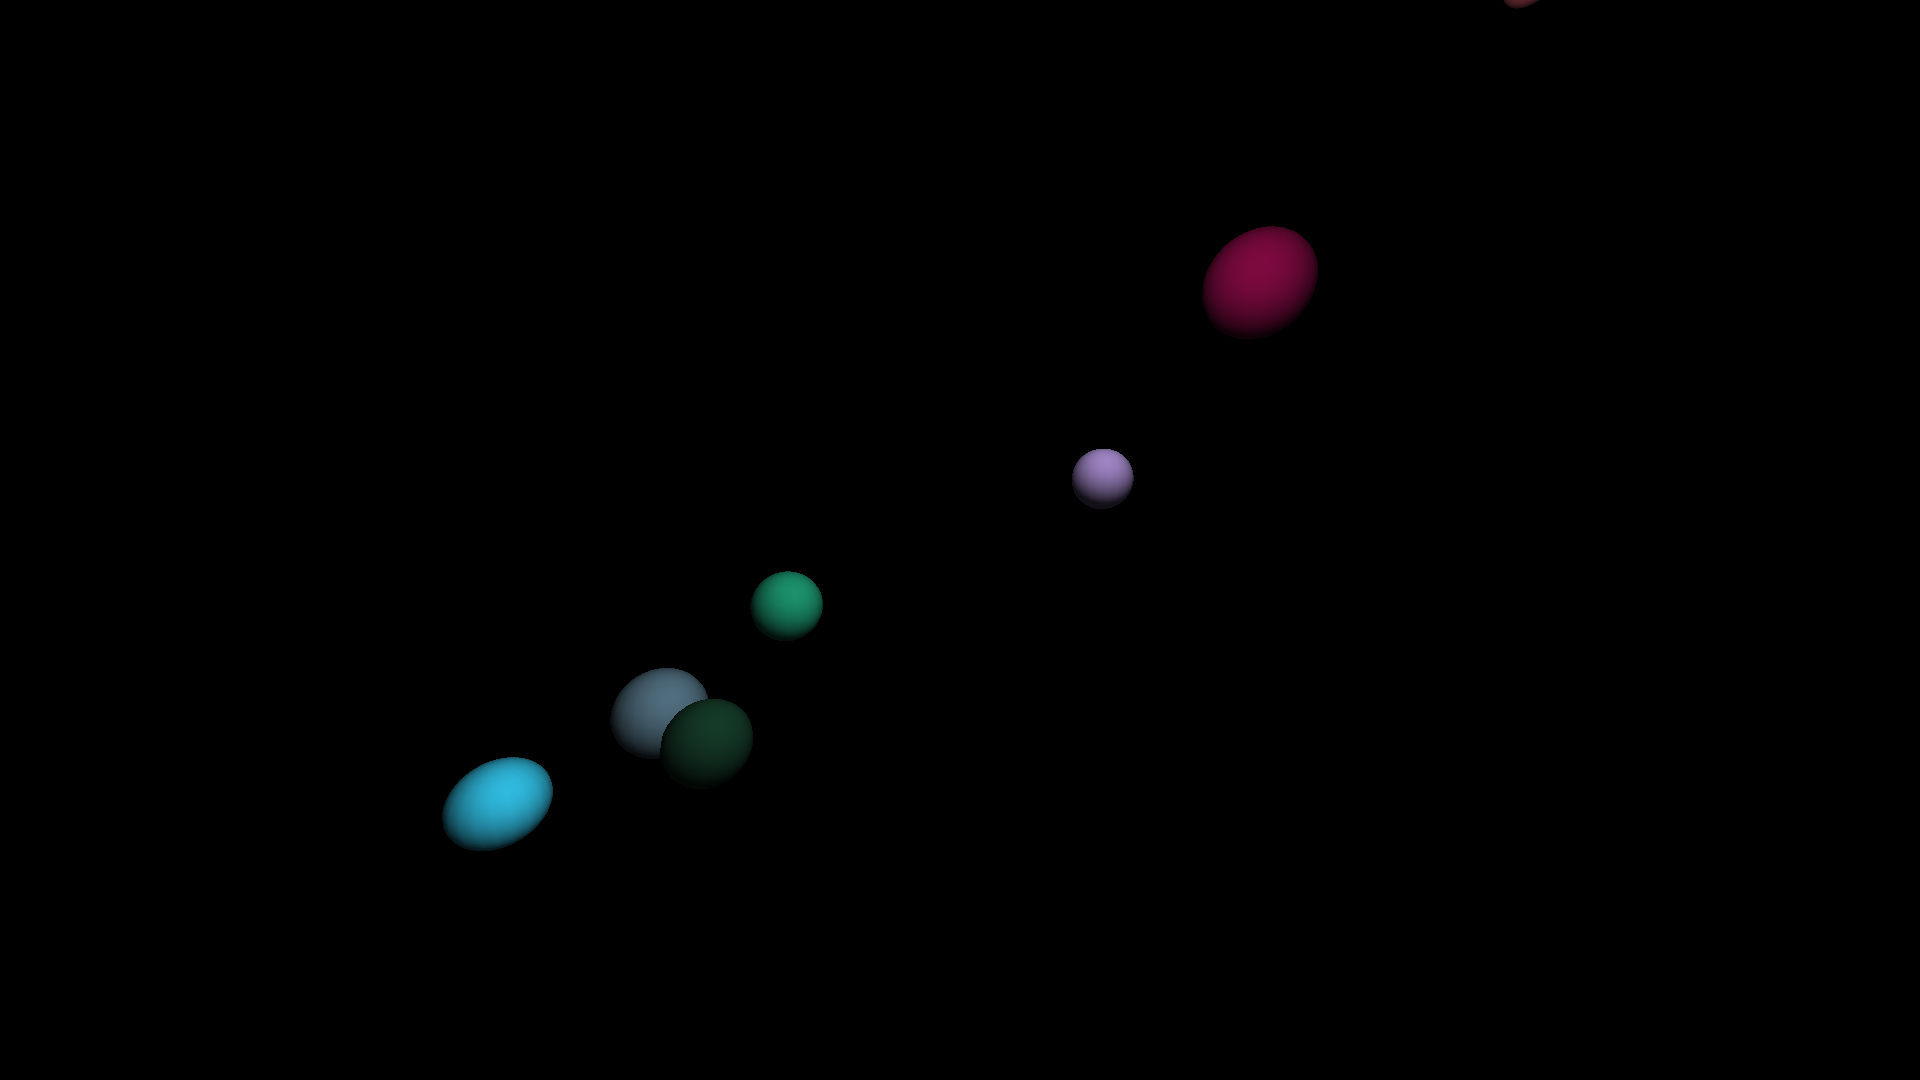
\includegraphics[width=\linewidth]{images/planets.png}

\subsection{Tim}
My work started with setting up a basic room using Three.js that could eventually be used as a home lobby connecting to the other rooms containing the experiences. Afterwards, I began working on user input to let the user move throughout the scenes. 

\subsubsection{Progress}
First, I created keyboard and mouse controls as that is the most accessible input scheme to use for basic testing of scenes. These controls are made using a Three.js tool called PointerLockControls which allows the user to move the camera using their mouse when the mouse pointer has been locked into the screen. For the keyboard movement, keydown and keyup event listeners are used to detect when a key has been pressed, figure out which key it is, and then perform the specific action associated with pressing that key, such as moving forward when the ‘W’ key or the up arrow is pressed. Using a Three.js 3D vector, I created a velocity vector to keep track of the x and z movement. When a key associated with movement is pressed, the correct amount of movement is applied to this velocity vector; for example, when the ‘S’ key is pressed, the “movement distance”, which is how far the user is moved each frame, is added to the z value of the velocity vector. This means, theoretically, it should be easy to produce movement in 45 degree angles when two keys are pressed with one moving in the x direction and the other in z. However, I needed some way of keeping track of when multiple keys have been pressed. This was done using a rather interesting solution making use of bitwise operations: 

\begin{lstlisting}
export function onKeyDown(event) {
 switch (event.keyCode) {
   case Key.Up:
   case Key.W:
     movingDirection |= Direction.Forward;
     break;
   case Key.Left:
   case Key.A:
     movingDirection |= Direction.Left;
     break;
   case Key.Down:
   case Key.S:
     movingDirection |= Direction.Backward;
     break;
   case Key.Right:
   case Key.D:
     movingDirection |= Direction.Right;
     break;
   default:
     break;
 }
}
\end{lstlisting}

This is called when the keydown event listener is fired. The movingDirection variable is simply an integer while Direction is a constant object exported from the control-utils file with the values used for detecting the correct movement:

\begin{lstlisting}
export const Direction = {
 Stopped: 0,
 Left: 1,
 Right: 2,
 Forward: 4,
 Backward: 8
};
\end{lstlisting}

These numbers are specifically chosen due to how they interact with each other when doing bitwise operations such as OR and AND. ORing these numbers will accomplish essentially the same thing as adding the values together. In the callback function for the keyup event listener, the AND and NOT operations are used:

\begin{lstlisting}
export function onKeyUp(event) {
 switch (event.keyCode) {
   case Key.Up:
   case Key.W:
     movingDirection &= ~Direction.Forward;
     break;
   case Key.Left:
   case Key.A:
     movingDirection &= ~Direction.Left;
     break;
   case Key.Down:
   case Key.S:
     movingDirection &= ~Direction.Backward;
     break;
   case Key.Right:
   case Key.D:
     movingDirection &= ~Direction.Right;
     break;
   default:
     break;
 }
}
\end{lstlisting}

This essentially does the same thing as subtracting the direction value from the total movingDirection number. In these cases, using bitwise operations is not necessary, but it is more efficient in terms of processing. When it becomes essential is when trying to figure out which keys are currently being pressed using this movingDirection number:

\begin{lstlisting}
const movingDistance = 100.0 * delta;

if ((movingDirection & Direction.Forward) === Direction.Forward) {
  velocity.z -= movingDistance;
}
if ((movingDirection & Direction.Backward) === Direction.Backward) {
  velocity.z += movingDistance;
}
if ((movingDirection & Direction.Left) === Direction.Left) {
  velocity.x -= movingDistance;
}
if ((movingDirection & Direction.Right) === Direction.Right) {
  velocity.x += movingDistance;
}
\end{lstlisting}

Due to the specific numbers that were chosen, when the movingDirection value is ANDed with the specific Direction value, it will result in that Direction value as long as it has yet to be “subtracted” away. For example, if the ‘W’ and ‘A’ key are pressed, then the movingDirection would be 4 (Direction.Forward) + 1 (Direction.Left), or 5.  5 ANDed with 4 results in 4, while 5 ANDed with 1 results in 1. However, 5 ANDed with 2 or 5 ANDed with 8 both result in 0. This works with every combination of these numbers to correctly detect which keys are currently pressed and update the position accordingly.

After the keyboard controls were implemented, I moved onto the touch controls. This was done using pointer and touch event listeners pointerdown, pointermove, and pointerup with similar event listeners touchstart, touchmove and touchend set in place to support browsers without the pointer listeners. The pointerdown callback simply stored where on the screen was touched. The pointermove callback is where the direction in which the user has moved their finger along the screen is calculated using the computeDirection method:

\begin{lstlisting}
const deltaX = ev.x - touchscreen.joystickOriginX;
const deltaY = ev.y - touchscreen.joystickOriginY;
computeDirection(deltaX, deltaY);
\end{lstlisting}

The variables deltaX and deltaY are calculated by simply finding the difference of delta of the x and y values in relation to the original touch point from the pointerdown event.

\begin{lstlisting}
export function computeDirection(deltaX, deltaY) {
  if (deltaX > 70) {
    velocity.x = -70;
  }
  if (deltaX < -70) {
    velocity.x = 70;
  }
  if (deltaY > 70) {
    velocity.z = -70;
  }
  if (deltaY < -70) {
    velocity.z = 70;
  }
  if ((deltaX <= 70 && deltaX >= -70) && (deltaY <= 70 && deltaY >= -70)) {
    joystick.style.transform = `translate(${deltaX}px,${deltaY}px)`;
    velocity.x = -deltaX;
    velocity.z = -deltaY;
  } else if ((deltaX <= 70 && deltaX >= -70) && (deltaY > 70)) {
    joystick.style.transform = `translate(${deltaX}px,70px)`;
  } else if ((deltaX <= 70 && deltaX >= -70) && (deltaY < -70)) {
    joystick.style.transform = `translate(${deltaX}px,-70px)`;
  } else if ((deltaY <= 70 && deltaY >= -70) && (deltaX > 70)) {
    joystick.style.transform = `translate(70px,${deltaY}px)`;
  } else if ((deltaY <= 70 && deltaY >= -70) && (deltaX < -70)) {
    joystick.style.transform = `translate(-70px,${deltaY}px)`;
  }
}
\end{lstlisting}

Computing the direction is as simple as using these deltaX and deltaY values as the x and z values in a velocity vector that is used to move the user. The first 4 if statements are there to set a boundary limit so that users wouldn't move insanely quick by swiping their finger a long distance across the screen quickly. The last if statement is for the general case in which the user keeps their finger within the 140 by 140 pixel range allocated for the joystick motion. Following the if statements are several else statements used for making the joystick animation much smoother when the user moves their finger past the bounded range.

To conclude my work, I added a method of opening the canvas in fullscreen mode for both keyboard and mouse as well as touch controls. On a desktop with keyboard and mouse, it will simply open in fullscreen when you click into the canvas. For mobile devices, there is a fullscreen button that launches fullscreen mode when pressed. To do this, I set up a control utils file with several utility methods that both the keyboard controls and touch controls could take from. The fullscreen code is rather straightforward using event listeners and built in dom calls such as requesting full screen and checking if it is currently active.

I also aided Jonathan with linking the two-eye immersive rendering with an Enter VR button I created, which is described in more detail in his section.

\subsubsection{Visuals}
Using touch controls in fullscreen.

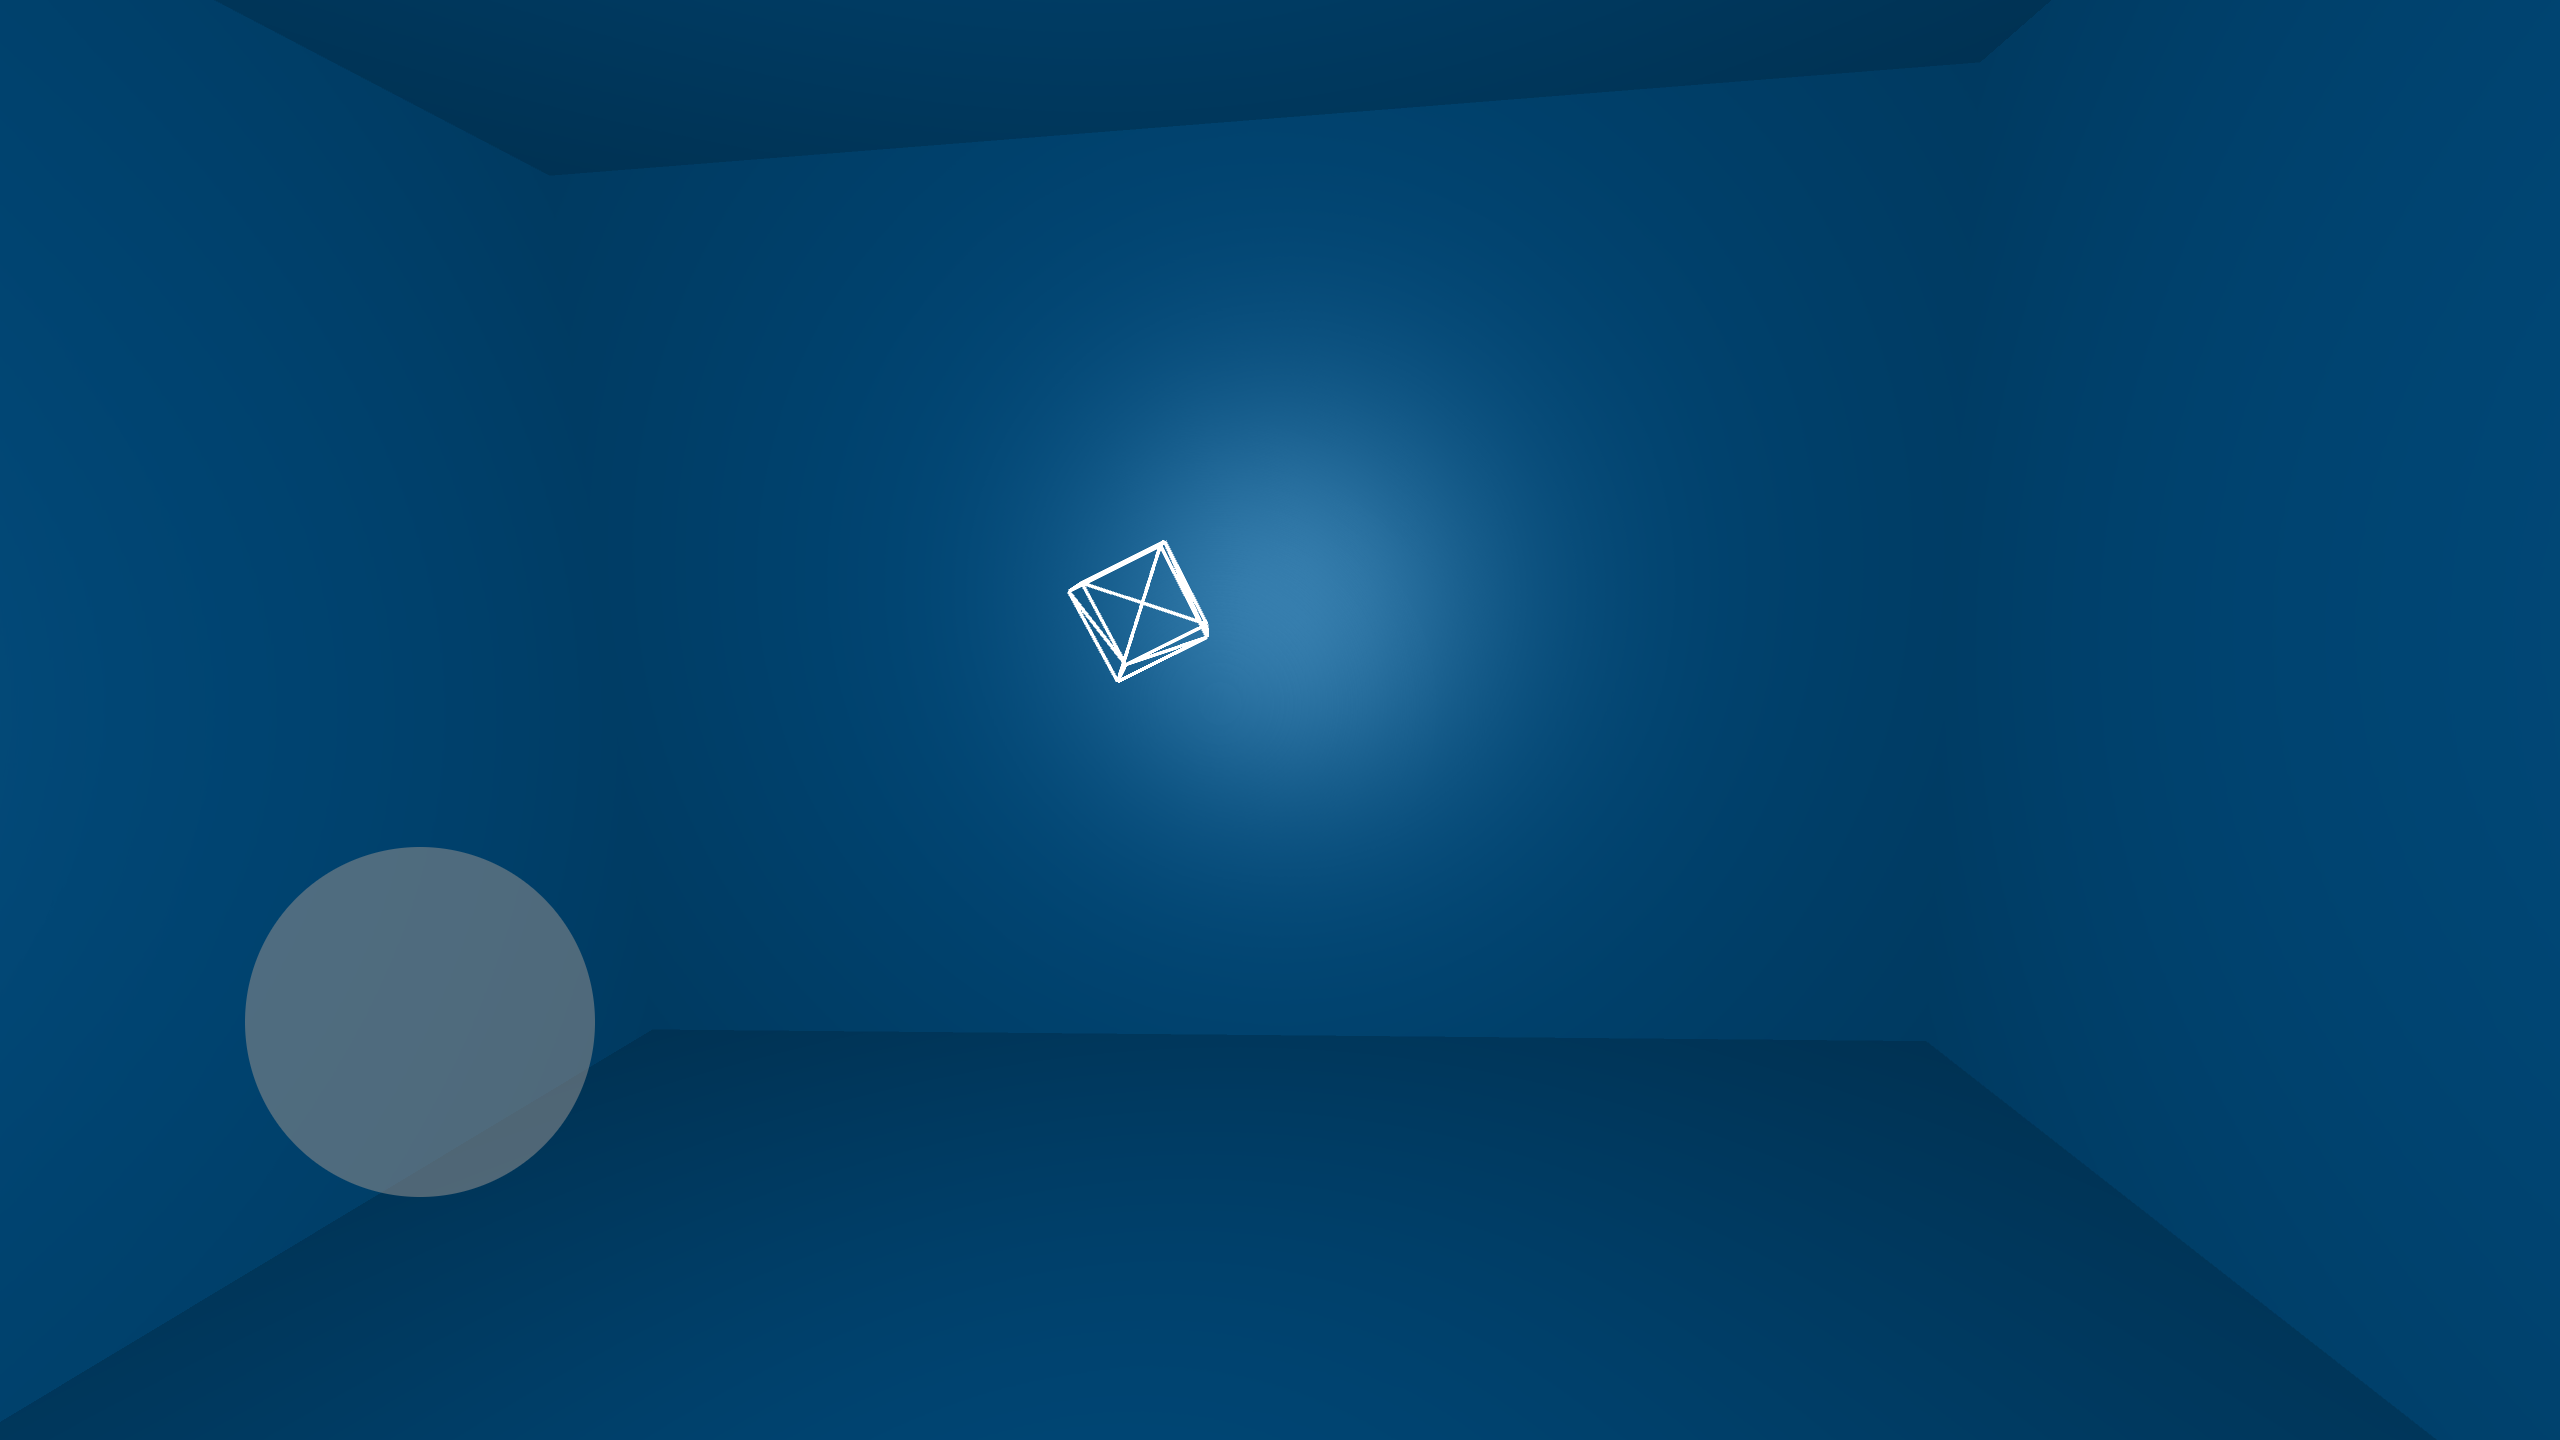
\includegraphics[width=\linewidth]{images/JoystickFullscreen.png}

Using touch controls in the browser window.

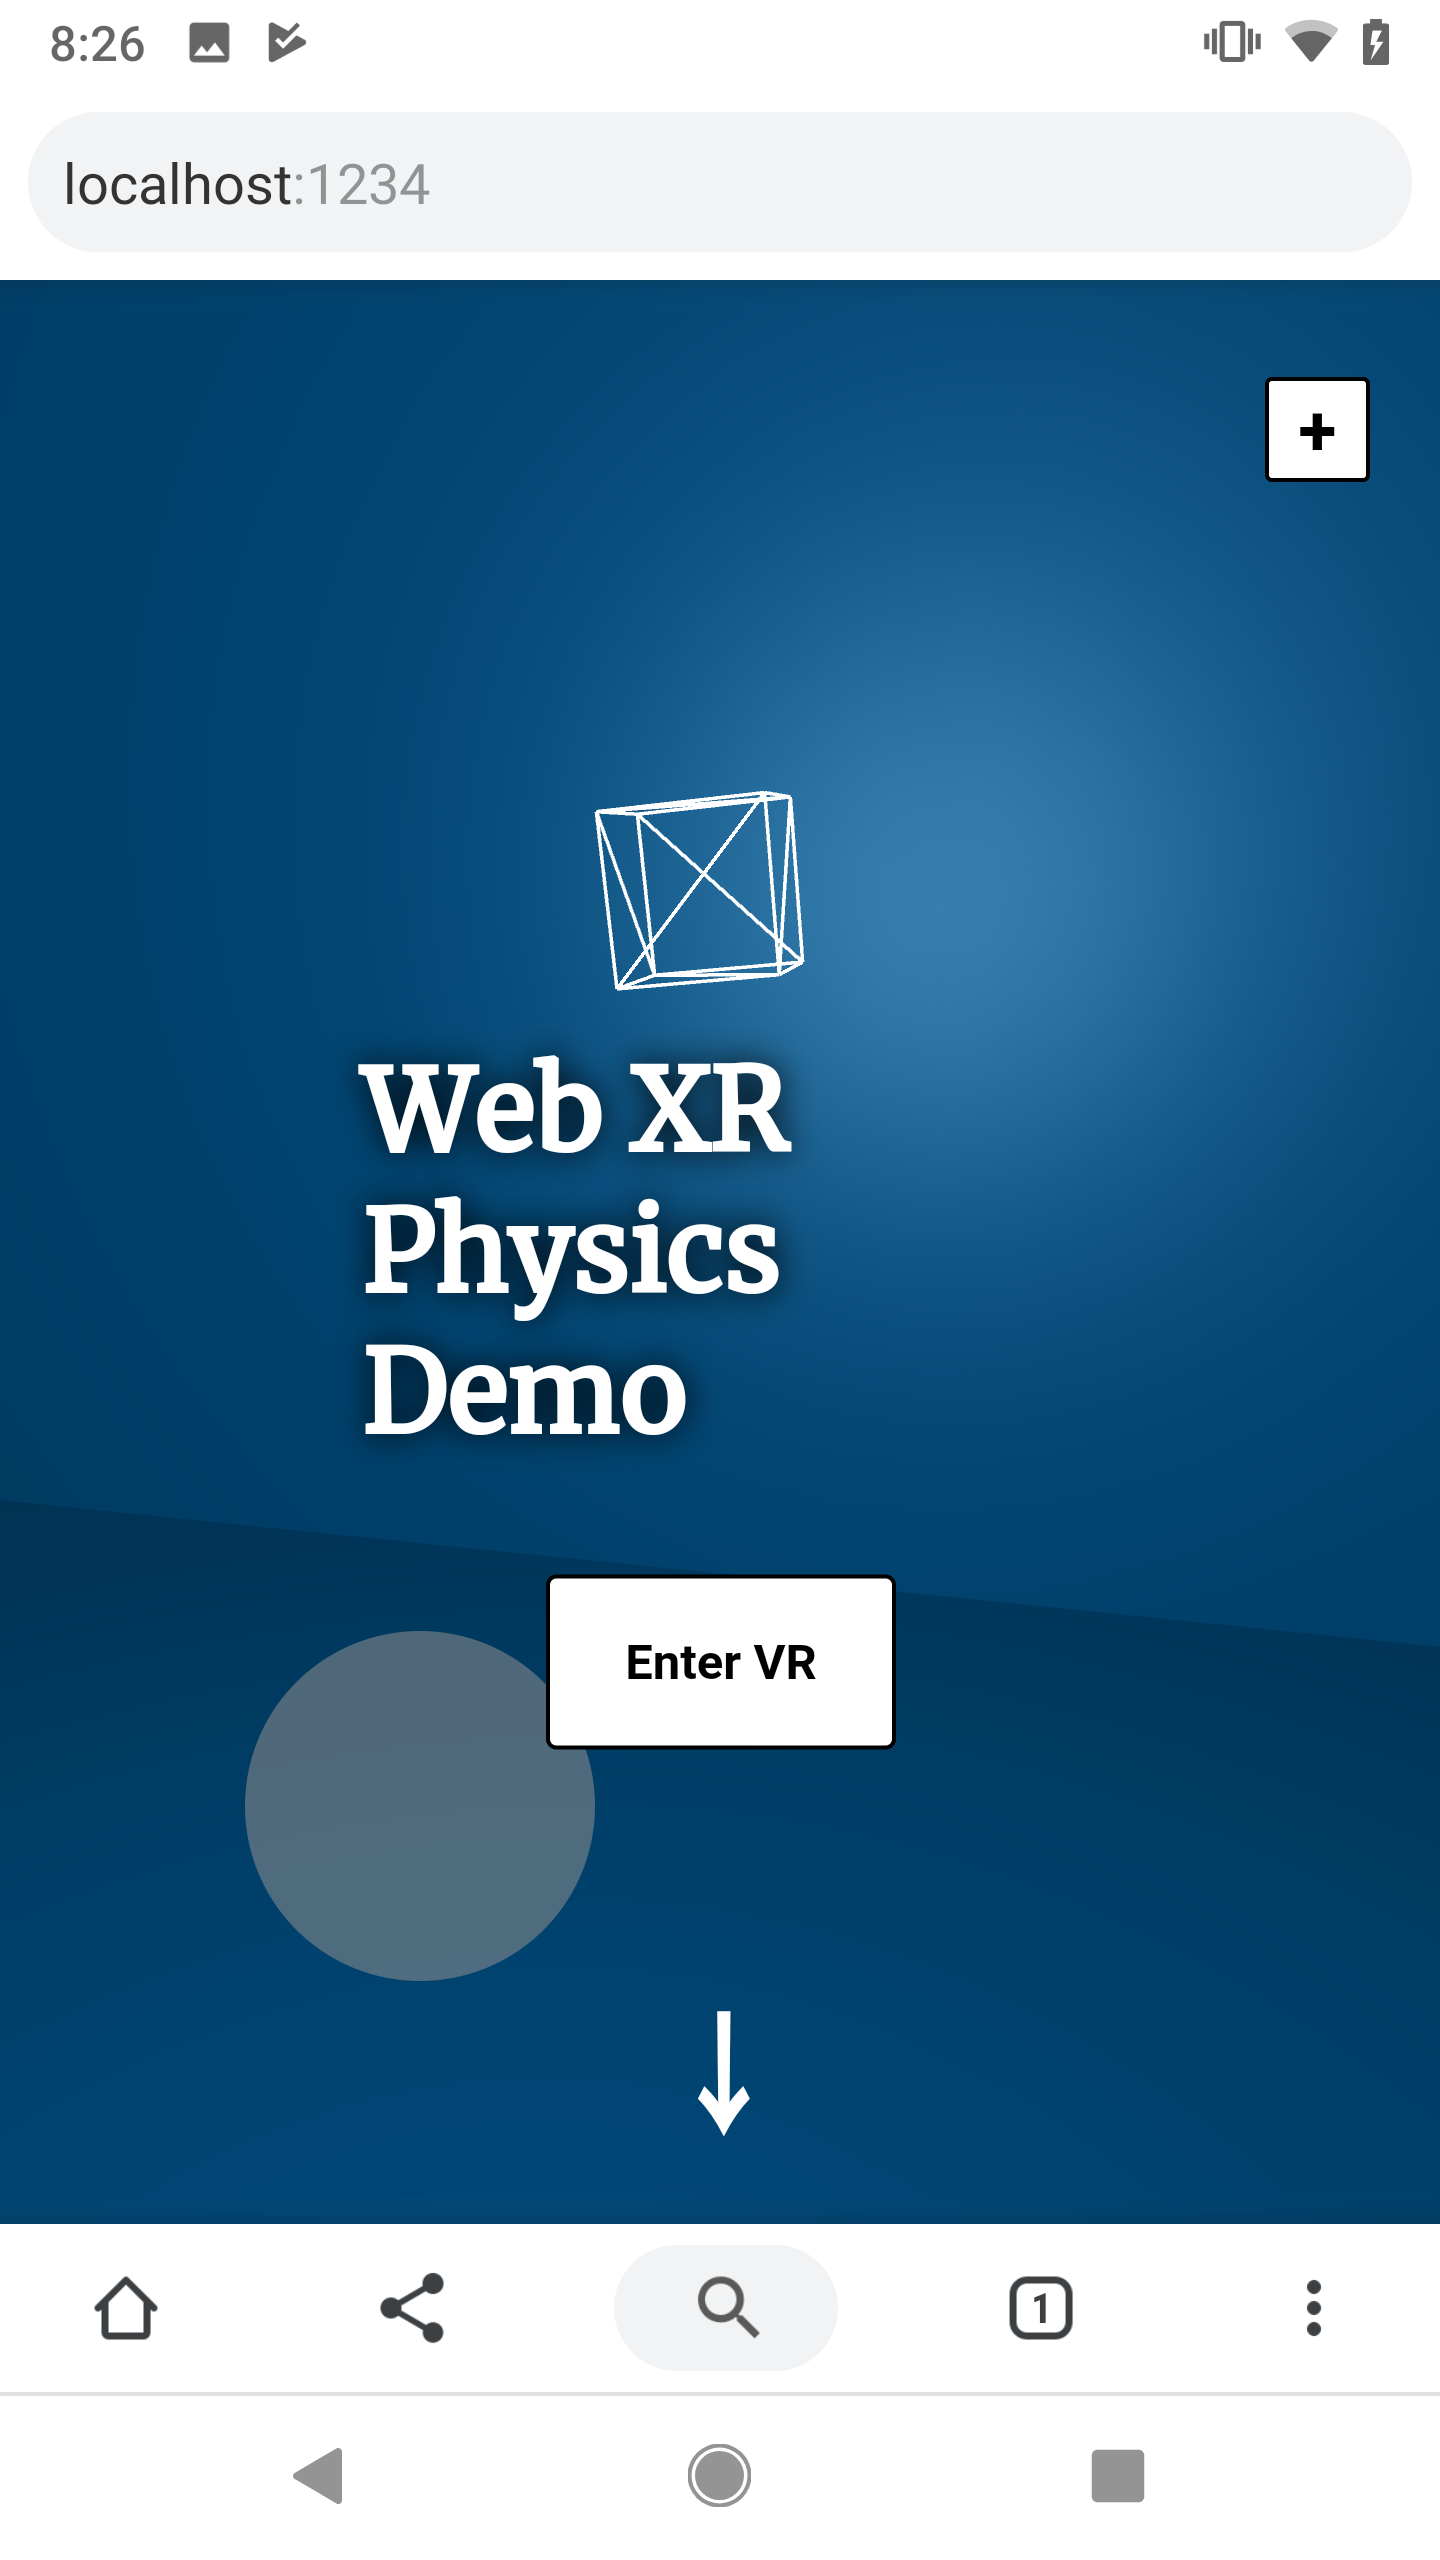
\includegraphics[width=0.35\linewidth]{images/JoystickWindow.png}

\subsection{Evan}
I've done some 3d modelling for the pendulum experience.  Currently, I have a planet surface, a pendulum, a table, a room with these objects placed and well lit, and a door.  All of these objects have few polygons fulfilling our goals of reaching a broad number of devices.

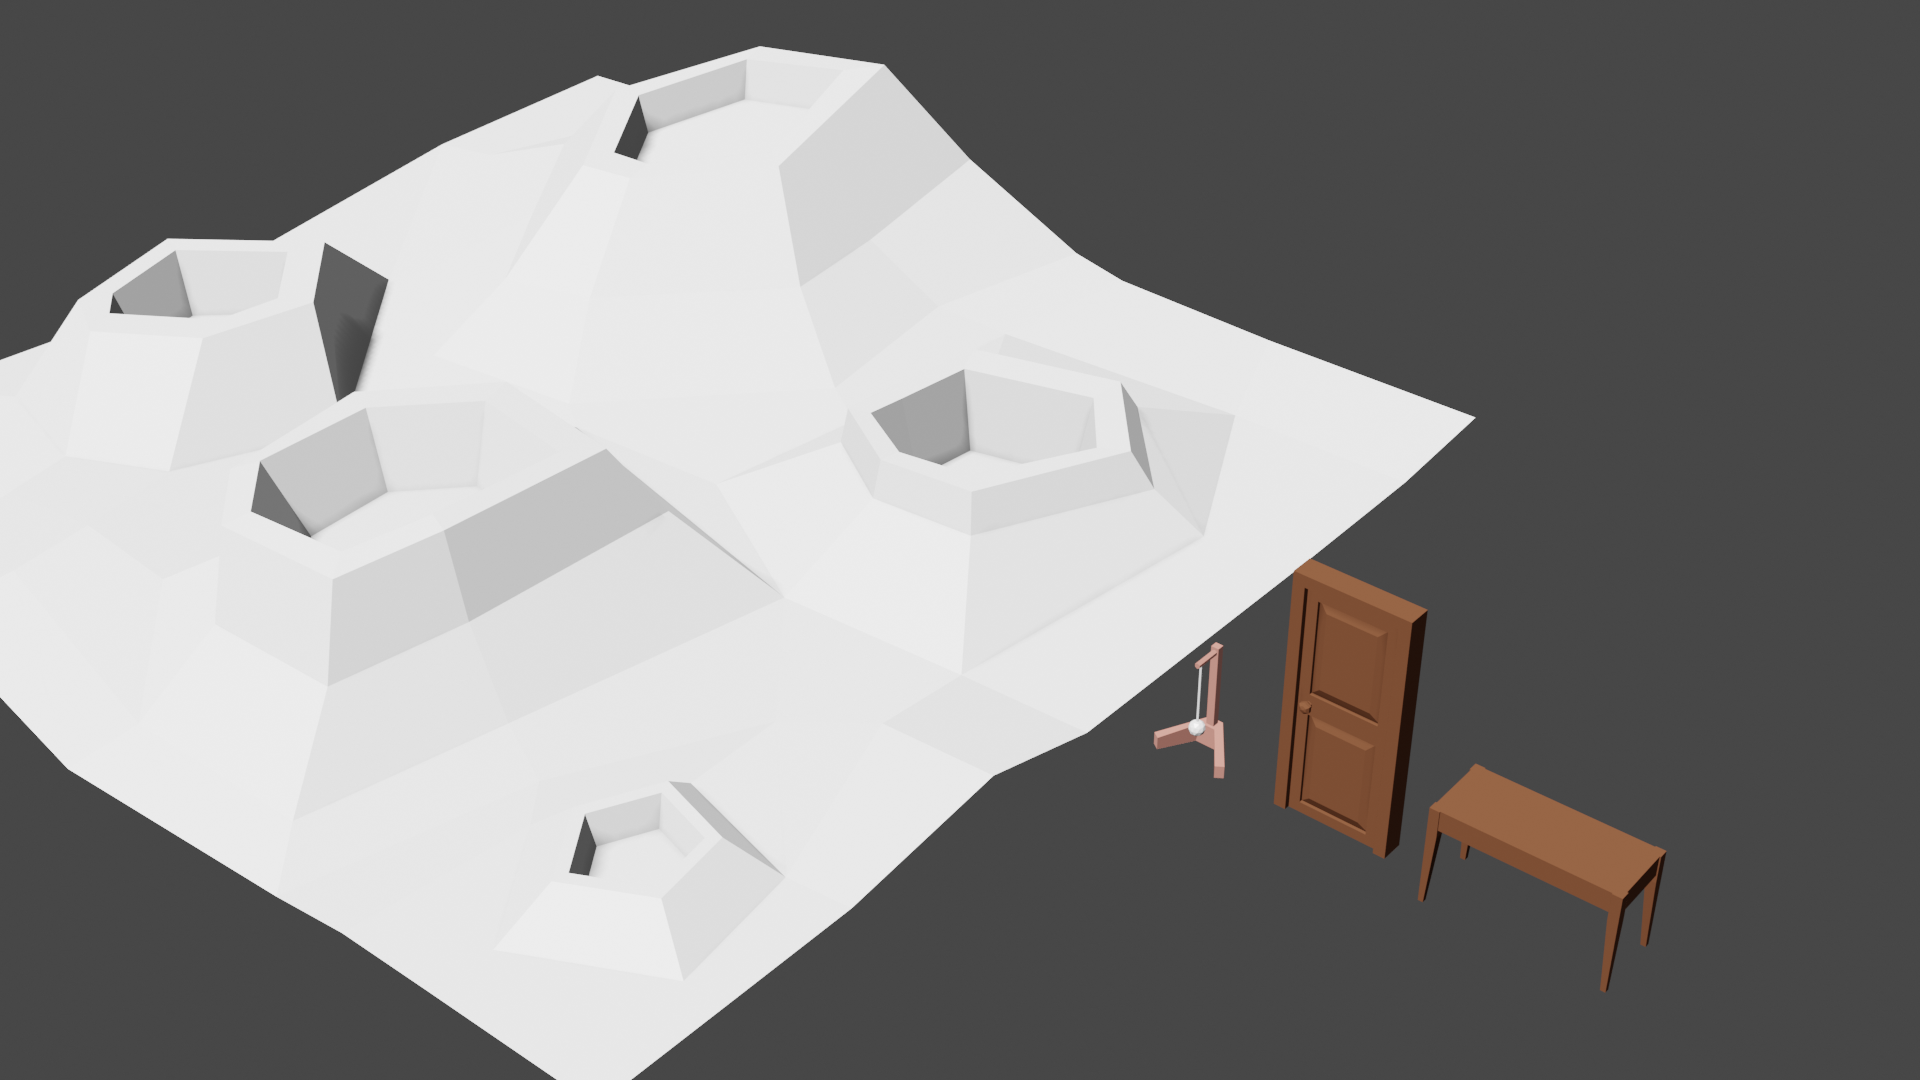
\includegraphics[width=\linewidth]{images/3d_objects.png}

The door will be how users navigate between rooms while in VR.  Currently, users can switch between rooms by exiting the immersive session and using normal links.  The possible navigation endpoints are in our router.js:

\begin{lstlisting}
const Routes = {
  get '/'() {
    return new HomeScene(renderer, camera);
  },
  get '/planets'() {
    return new PlanetsScene(renderer, camera);
  },
  get '/pendulums'() {
    return new PendulumScene(renderer, camera);
  }
};
\end{lstlisting}

Each link has an event listener that intercepts the navigation and switches scenes which will be easy to replace with the doors when we fix the alignment.

\begin{lstlisting}
// Navigation using links
for (const el of document.links) {
  el.addEventListener('click', (e) => {
    e.preventDefault(); // Stop the browser from navigating to the link's location.
    e.stopPropagation();
    navigate((new URL(el.href)).pathname);
  });
}
// Navigation using doors will look something like:
for (let door of doors) {
    door[Interactions] = {
        select(closeness, {distance, point, face, faceIndex, uv}) {
          navigate('/'); // Navigate to the home room
        }
    };
}
\end{lstlisting}

I also did the initial website styling including the animated arrow, full width and height first page.

My latest work has been building the framework for responding to the 3d equivalents of click and hover events.  Objects can have callbacks for select and hover.  While these are functional, I'm still figuring out why the object that receives the interaction (in yellow) is not the object that appears under the virtual cursor (light blue):

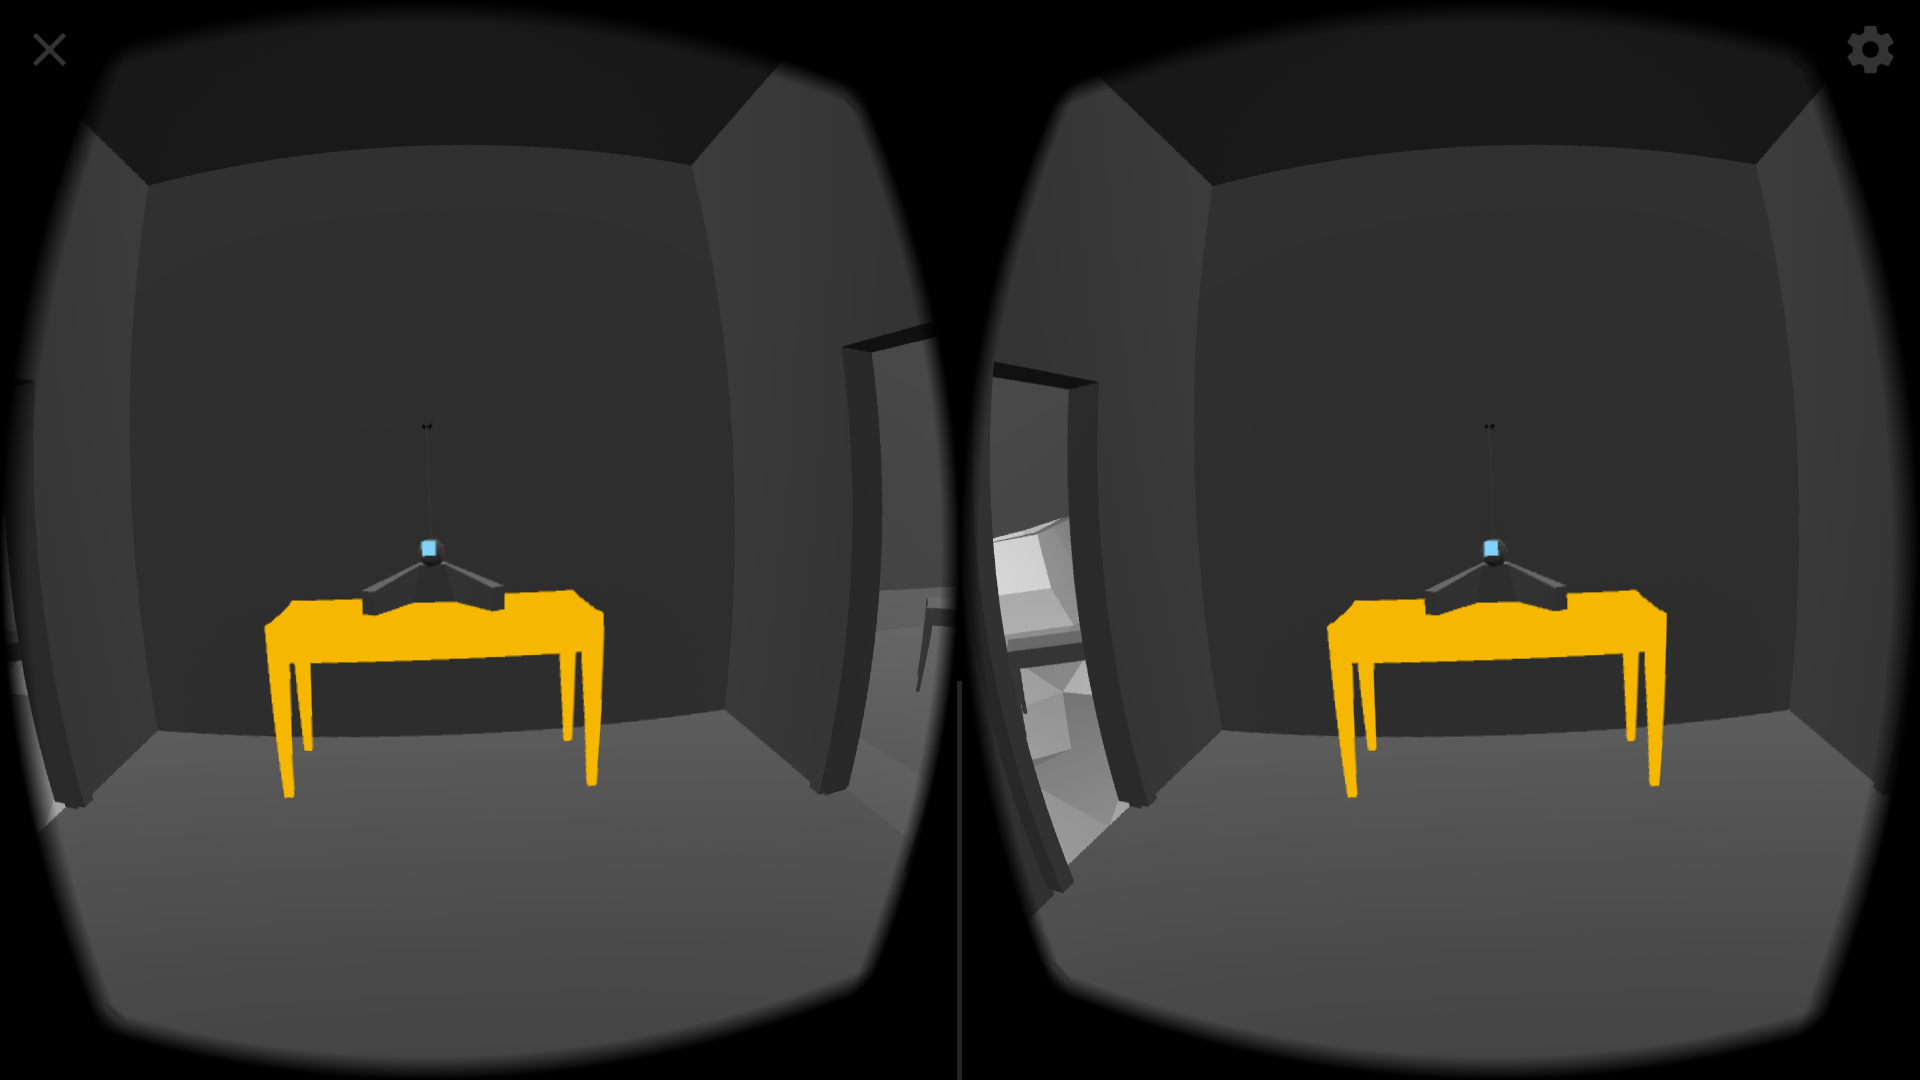
\includegraphics[width=\linewidth]{images/pendulum-select_offset.png}


\subsection{Jonathan}
Over the last few weeks I have been responsible for setting up the Three.js graphical back-end and implementation of the WebXR API in conjunction with the Three.js renderer. My work in Three.js included setting up boilerplate code, a shared parent class among the experiences and a unified animation handler between those rooms. For the WebXR API I was tasked with XR device validation and XR session initialization. This enabled the site to check for XR devices and then set up a magic window or immersive VR rendering session. Finally, I worked to set up event listeners for a VR button that allowed the user to activate/create an immersive VR session on click.

    \subsubsection{Progress}
    
    For the first couple of weeks, I spent my time tinkering with the Three.js code looking for a way to make sure that all the experience rooms would cooperate with each other in runtime. Along with Brooks, we decided on a structure in which all experience rooms are derived from one parent class that shares a renderer and animation handler. This allows us to easily switch between different rooms by constructing them from the parent class on each room switch event. The shared renderer also provides a seamless transition between experience rooms and the unified animation handler ensures that each new room can easily begin rendering frames on creation. 
    
    While setting up the unified animator, we ran into an issue where the animation loops of previous rooms continued executing even after the room had changed. This was solved by setting an isActive value for each room instance. Later on, I added a restart animation function that would stop execution of the current animation loop then start it up again. This was implemented in response to an issue where XR sessions would automatically end the current animation loop. For some XR sessions, it's required that the animation loop is manually started up again on its creation. There were some other cases though where the XR session would start a second animation loop. The cancel animation frame code was added to handle events in which a frame had already been in the render loop.
    \begin{lstlisting}
  /**
   * Override this to handle animating objects in your scene.
   * @param {number} delta time since last scene update
   */
  animate(delta) {
    return delta;
  }

  /**
   * Call this to begin animating your frame.
   */
  startAnimation() {
    this._animationCallback();
  }

  _restartAnimation = () => {
    if (this.frame) window.cancelAnimationFrame(this.frame);
    this._animationCallback();
  };

  _animationCallback = (timestamp, xrFrame) => {
    if (this.isActive) {
      // Update the objects in the scene that we will be rendering
      const delta = this.clock.getDelta();
      this.animate(delta);
    \end{lstlisting}
    
    The majority of my time over the last few weeks was spent implementing the WebXR API. There were many challenges to overcome. First of all was the instability of the API and its unreliable polyfill. Under the direction of the client, I started this process using the WebXR polyfill. This was a mistake. The polyfill is not nearly as reliable as the most current version of WebXR. Though it is a polyfill, oftentimes the functions I needed to call were unsupported and out of date. After some discussion with the client, I stopped using the polyfill.
    
    The up-to-date API was not without its issues. As it is brand new and unstable, we are required to use the most up-to-date version of Chrome Dev/Canary for testing/deployment and often, many of the code snippets we write are unreliable and may be unusable at any time. For this reason, we are constantly having to keep an eye on the WebXR API and Chrome updates.
    
    The WebXR session validation is a multi-step process that begins with checking if the current device is capable of non-immersive sessions. A non-immersive session is one in which XR properties of the device are read, but are only used in a single rendering context. This is also called magic window rendering, a session primarily used on mobile devices. Most modern mobile devices can support these types of sessions and will pass the checks that I have written.
    
    Before a magic window session is created, a new xrpresent rendering context needs to be created. Normally, a WebGL rendering context is used and this is what our main rendering canvas uses. Unfortunately, once a rendering context has been attached to a canvas, it can no longer be changed. Instead, a new canvas is created with the correct rendering context and added to the DOM. Once that canvas has been created, the WebXR API navigator makes a request for a non-immersive session using the rendering context we've just created. 
    \begin{lstlisting}
/**
 * Checks for magic window compatibility
 */
async function xrValidateMagicWindow() {
  // Ensure that there isn't already a magic window
  if (!XR.magicWindowCanvas) {
    XR.magicWindowCanvas = document.createElement('canvas');
    XR.magicWindowCanvas.setAttribute('id', 'vr-port');
    XR.magicWindowCanvas.setAttribute('name', 'magic-window');
    canvas.parentNode.insertBefore(XR.magicWindowCanvas, canvas);
  }
  XR.magicWindowCanvas.width = window.innerWidth;
  XR.magicWindowCanvas.height = window.innerHeight;

  // Set canvas rendering context to xrpresent
  const xrMagicWindowContext = XR.magicWindowCanvas.getContext('xrpresent');

  try {
    XR.session = await navigator.xr.requestSession({ outputContext: xrMagicWindowContext });
    canvas.style.display = 'none';
    xrOnSessionStarted();
  } catch (reason) {
    XR.magicWindowCanvas.style.display = 'none';
    console.log(`Device unable to support magic window session : ${reason}`);
  }
}
    \end{lstlisting}
    
    When requesting an immersive session, the process is similar to magic window validation.
    \begin{lstlisting}
/**
 * Gets an immersive two eye view xr session when the 'ENTER XR' button has been pressed
 */
async function xrOnRequestSession() {
  // Create a mirror canvas for rendering the second eye
  const xrMirrorCanvas = document.createElement('canvas');
  const xrMirrorContext = xrMirrorCanvas.getContext('xrpresent');
  xrMirrorCanvas.setAttribute('id', 'mirror-canvas');

  // Add the mirror canvas to our XR object and the document.
  XR.mirrorCanvas = xrMirrorCanvas;
  document.body.appendChild(xrMirrorCanvas);

  // Attempt to create an XR session using the mirror canvas and the connected device
  try {
    XR.session = await navigator.xr.requestSession({ mode: 'immersive-vr', outputContext: xrMirrorContext });
    xrOnSessionStarted();
  } catch (err) {
    console.error(`Error initializing XR session : ${err}`);
  }
}
    \end{lstlisting}
    
    Once the XR session has been created, I export an XR object that contains all the necessary information to render a single frame. The session object, the frame of reference from which XR input is written and the two rendering canvases.
    \begin{lstlisting}
export const XR = {
  session,
  immersiveRefSpace,
  nonImmersiveRefSpace,
  magicWindowCanvas,
  mirrorCanvas
};
    \end{lstlisting}
    
    Finally, in the unified animator, I query the reference space for its pose. The pose holds all the XR views, these views hold their rendering viewports and the transformation matrices for each XR object in the scene. I used this information to manually update the three.js camera and scene matrices to reflect the positioning of the XR device.
    \begin{lstlisting}
for (let i = 0; i < pose.views.length; i++) {
  const view = pose.views[i];
  const viewport = XR.session.renderState.baseLayer.getViewport(view);
  const viewMatrix = new Matrix4().fromArray(view.viewMatrix);

  this.renderer.context.viewport(
    viewport.x,
    viewport.y,
    viewport.width,
    viewport.height
  );

  // Update user position if touch controls are in use with magic window.
  if (XR.magicWindowCanvas && XR.magicWindowCanvas.hidden === false) {
    updateTouchPosition(viewMatrix);
    this._translateViewMatrix(viewMatrix, userPosition);
    } else {
      this._translateViewMatrix(viewMatrix, new Vector3(0, 0, 0));
    }

    this.camera.matrixWorldInverse.copy(viewMatrix);
    this.camera.projectionMatrix.fromArray(view.projectionMatrix);
    this.scene.matrix.copy(viewMatrix);

    this.scene.updateMatrixWorld(true);
    this.renderer.render(this.scene, this.camera);
    this.renderer.clearDepth();
}
    \end{lstlisting}
    
    \subsubsection{Visuals}
    Magic Window
    
    
\includegraphics[width=\linewidth]{images/MagicWindow.png}
    
    Immersive View
    
    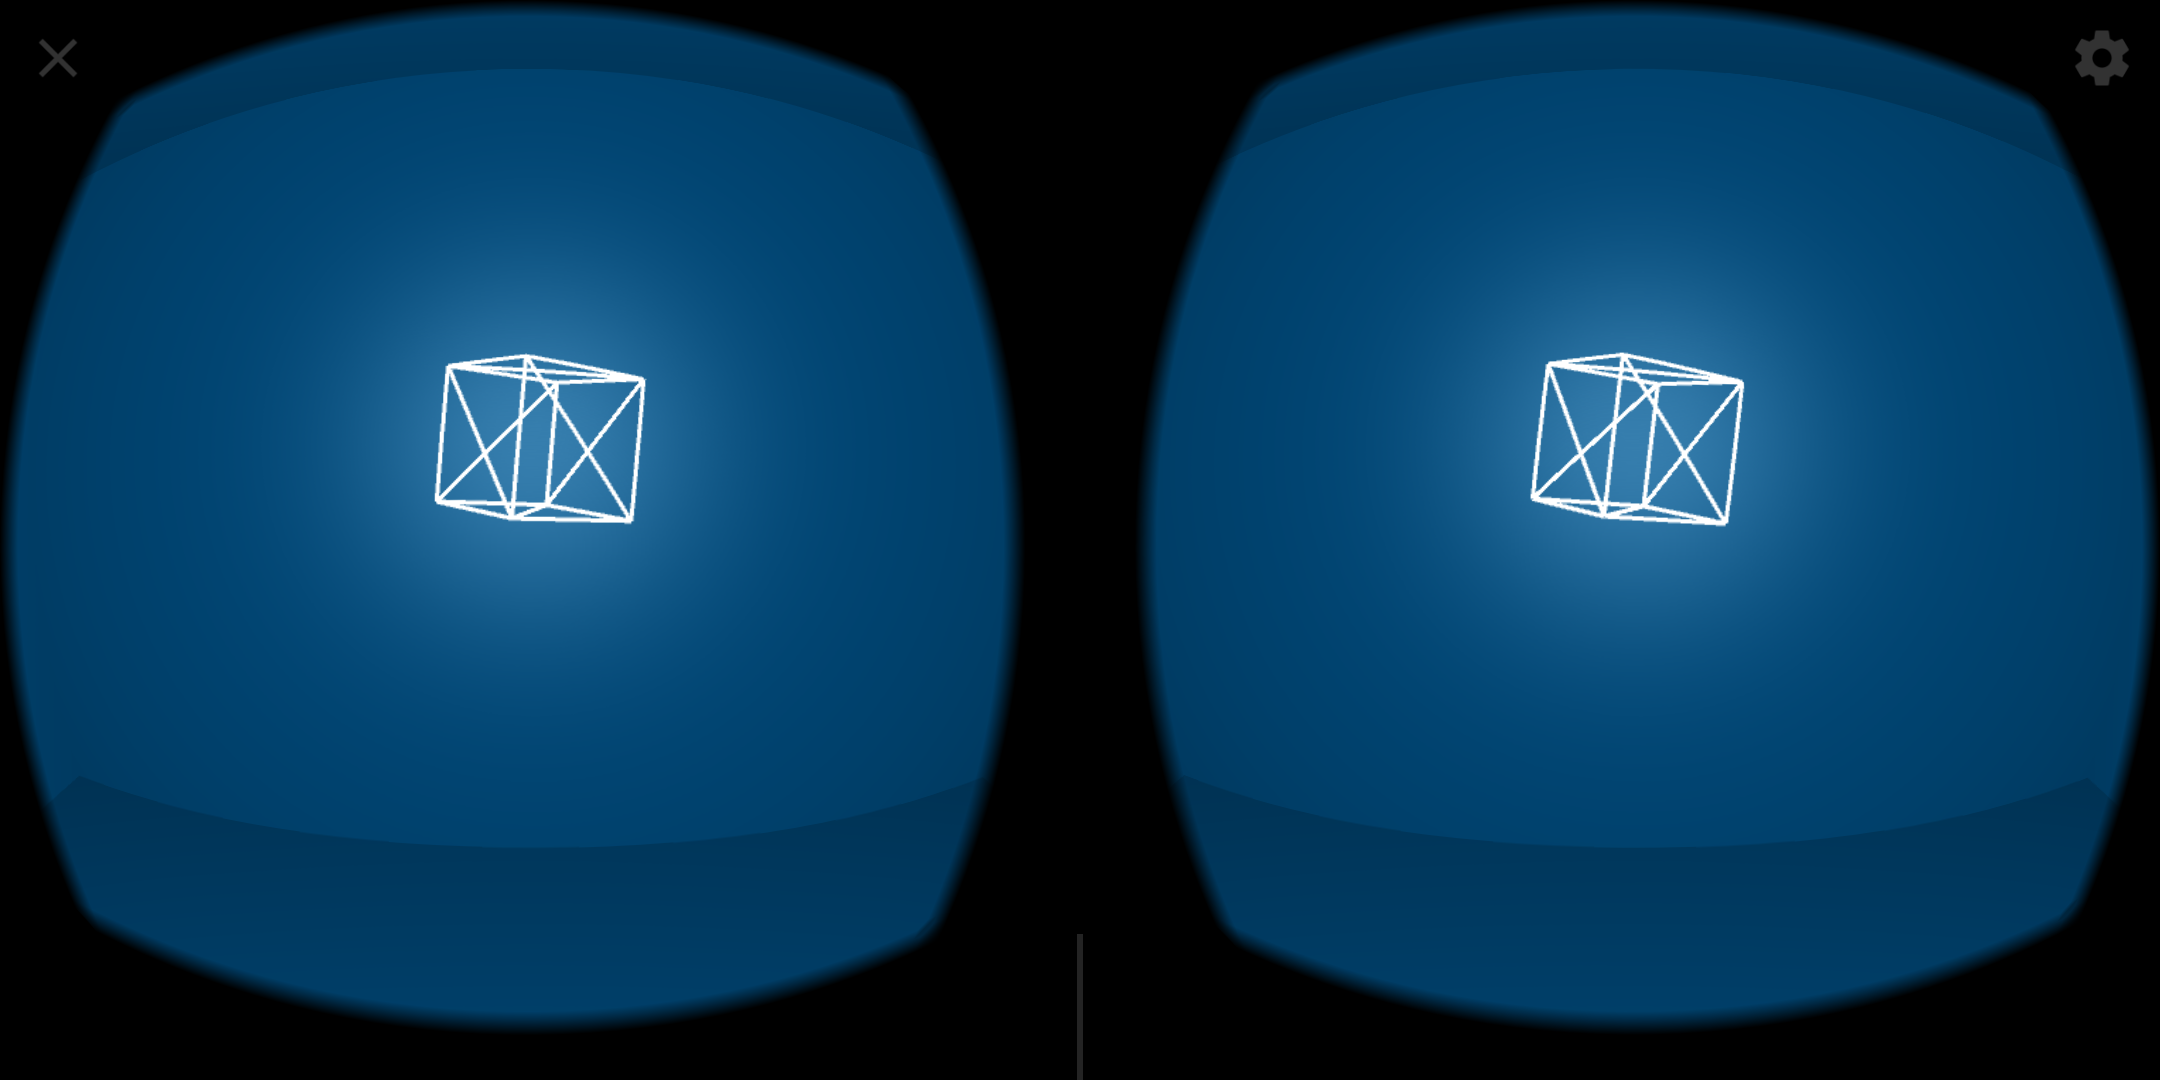
\includegraphics[width=\linewidth]{images/ImmersiveView.png}
    
\subsection{Brandon}
   For the couple of weeks I have been tasked for setting up Cannon.js. My work started with setting up a basic room using Three.js that could later used when setting up a Lightweight 3D physics for the web. I began with the creation of a cannon world object.
   
   \subsubsection{Progress}
   First, I begin creating a cannon world that is the physics hub that manage objects and simulation. Then I set the gravity to be in the negative y direction and I added a broadphase algorithm to the world so it can easily find colliding bodies. This will set up the physics world and the next part is adding objects to it. The bodies are built once you define a shape, a rigid body using the shape and other physical properties needed, and then add the body to the world. I created a spherical shape with a radius of 1 so it can be put into a rigidbody before it can move and collide. Next I create a rigidbody and set the body mass to 1 so it makes the sphere dynamic. If the mass is set to zero it becomes static amd static don't collie with other static bodies. While dynamic ones collie with all other bodies. Lastly, I add the body to the world so it will move according to the forces it is subject to, and collide with other objects:
   
   \begin{lstlisting}
    const world = new CANNON.World();
    world.gravity.set(0,-15,0);
    world.broadphase = new CANNON.NaiveBroadphase();
    const radius = 1
    const sphereBody = new CANNON.Body(
      {
        mass: 1,
        position: new CANNON.Vec3(1, 0, 0),
        shape: new CANNON.Sphere(radius)
      }
    );
    sphereBody.position.set(0, 5, -5);
    this.world.add(sphereBody);
   \end{lstlisting}
   
   This will create the plane shape, and then the body. I give the body zero mass, this will make sure the ground body to become static. The orientation of the plane I set in a 90 degree angle: 
   
   \begin{lstlisting}
    const groundShape = new CANNON.Plane();
    const groundBody = new CANNON.Body({ mass: 0 });
    groundBody.addShape(groundShape);
    groundBody.quaternion.setFromAxisAngle(new CANNON.Vec3(1, 0, 0), -Math.PI / 2);
    groundBody.position.set(0, -8, 0);
    this.world.addBody(groundBody);
    this.world.add(sphereBody);
    const body = sphereBody;
    return body;
   \end{lstlisting}
    
    After we have initialized the static ground plane and a dynamic sphere. I then set a time step for Cannon.js. Cannon.js uses a computation algorithm to called integrators to simulate the physics equations at a discrete points of time. This step at least 60hz or 1/60 seconds to begin the simulation loop:
   \begin{lstlisting}
   animate() {
   this.updatePhysics();
   this.ball.position.copy(this.body.position);
   this.ball.quaternion.copy(this.body.quaternion);
   }
   \end{lstlisting} 
   
   \subsubsection{Visuals}
   Sphere position set.
   
   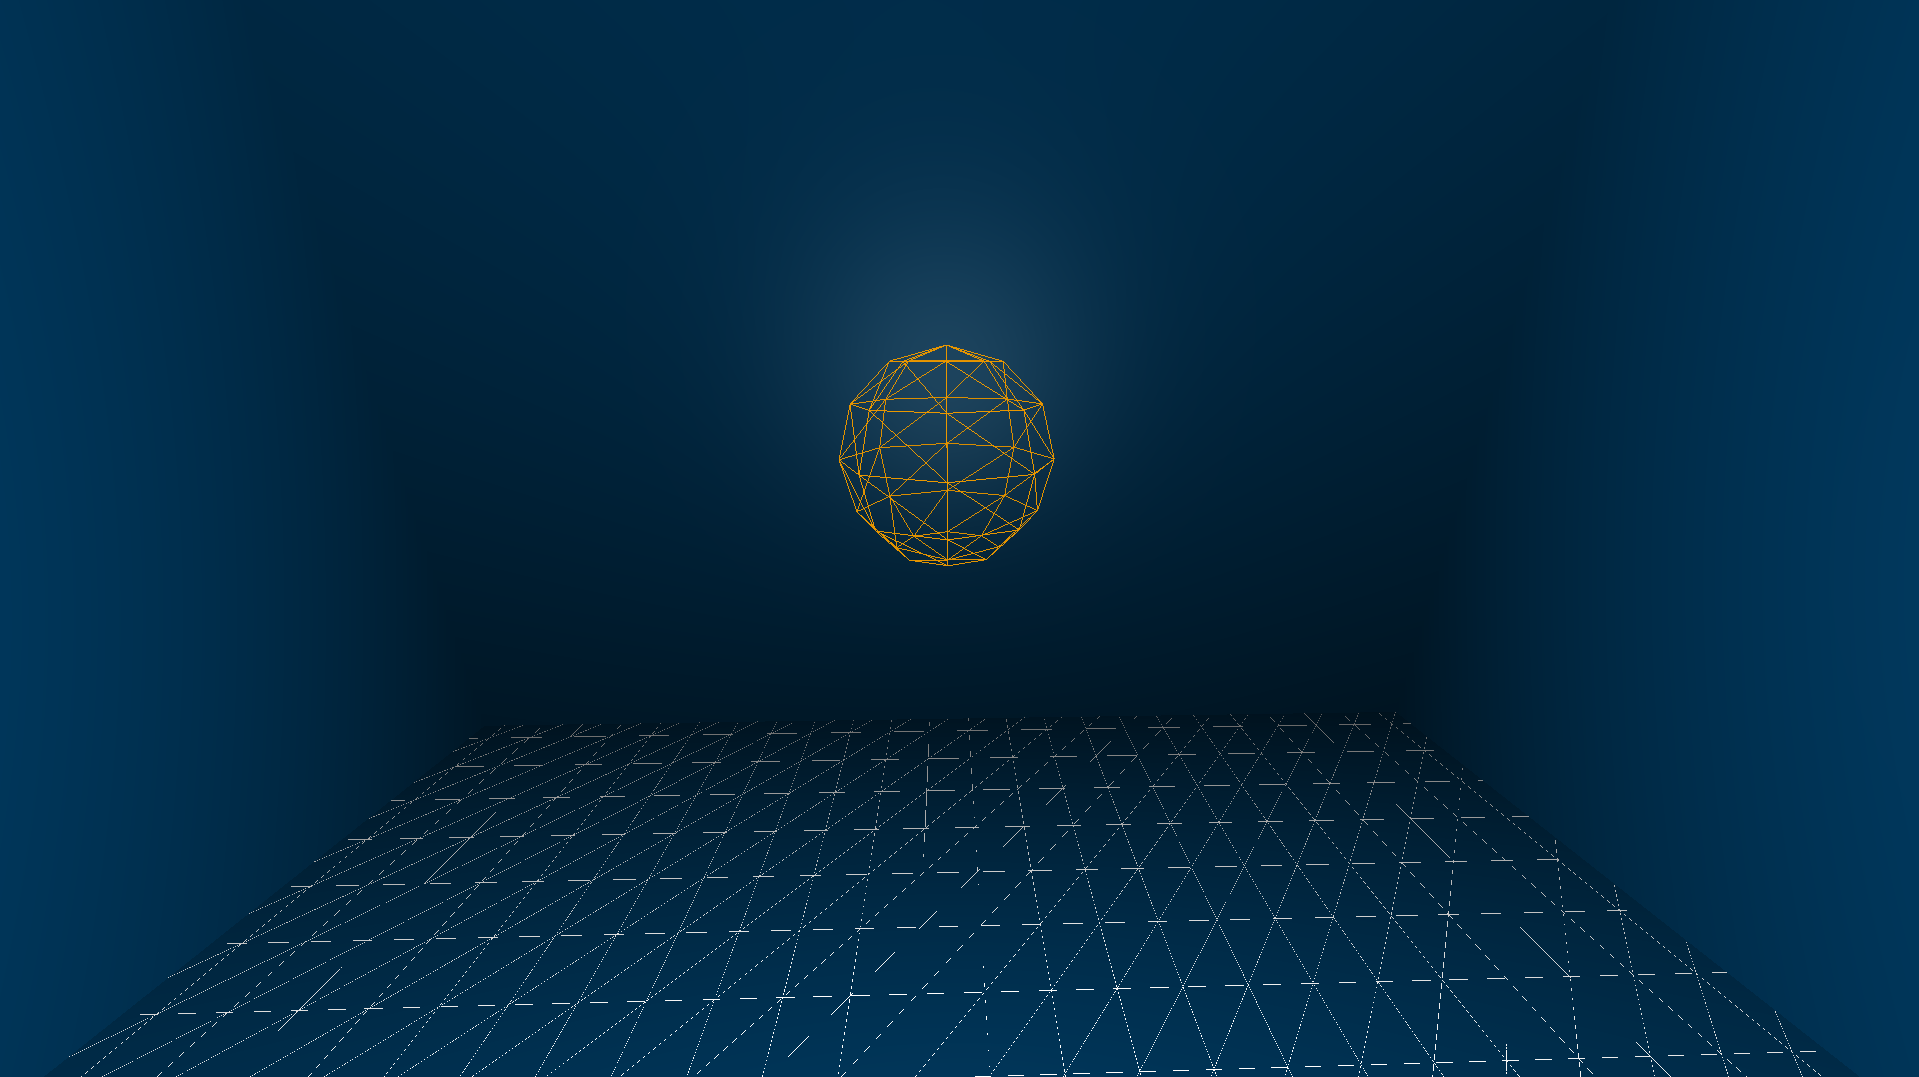
\includegraphics[width=\linewidth]{images/Cannonjs.png}
   
   Sphere simulate drop.
   
   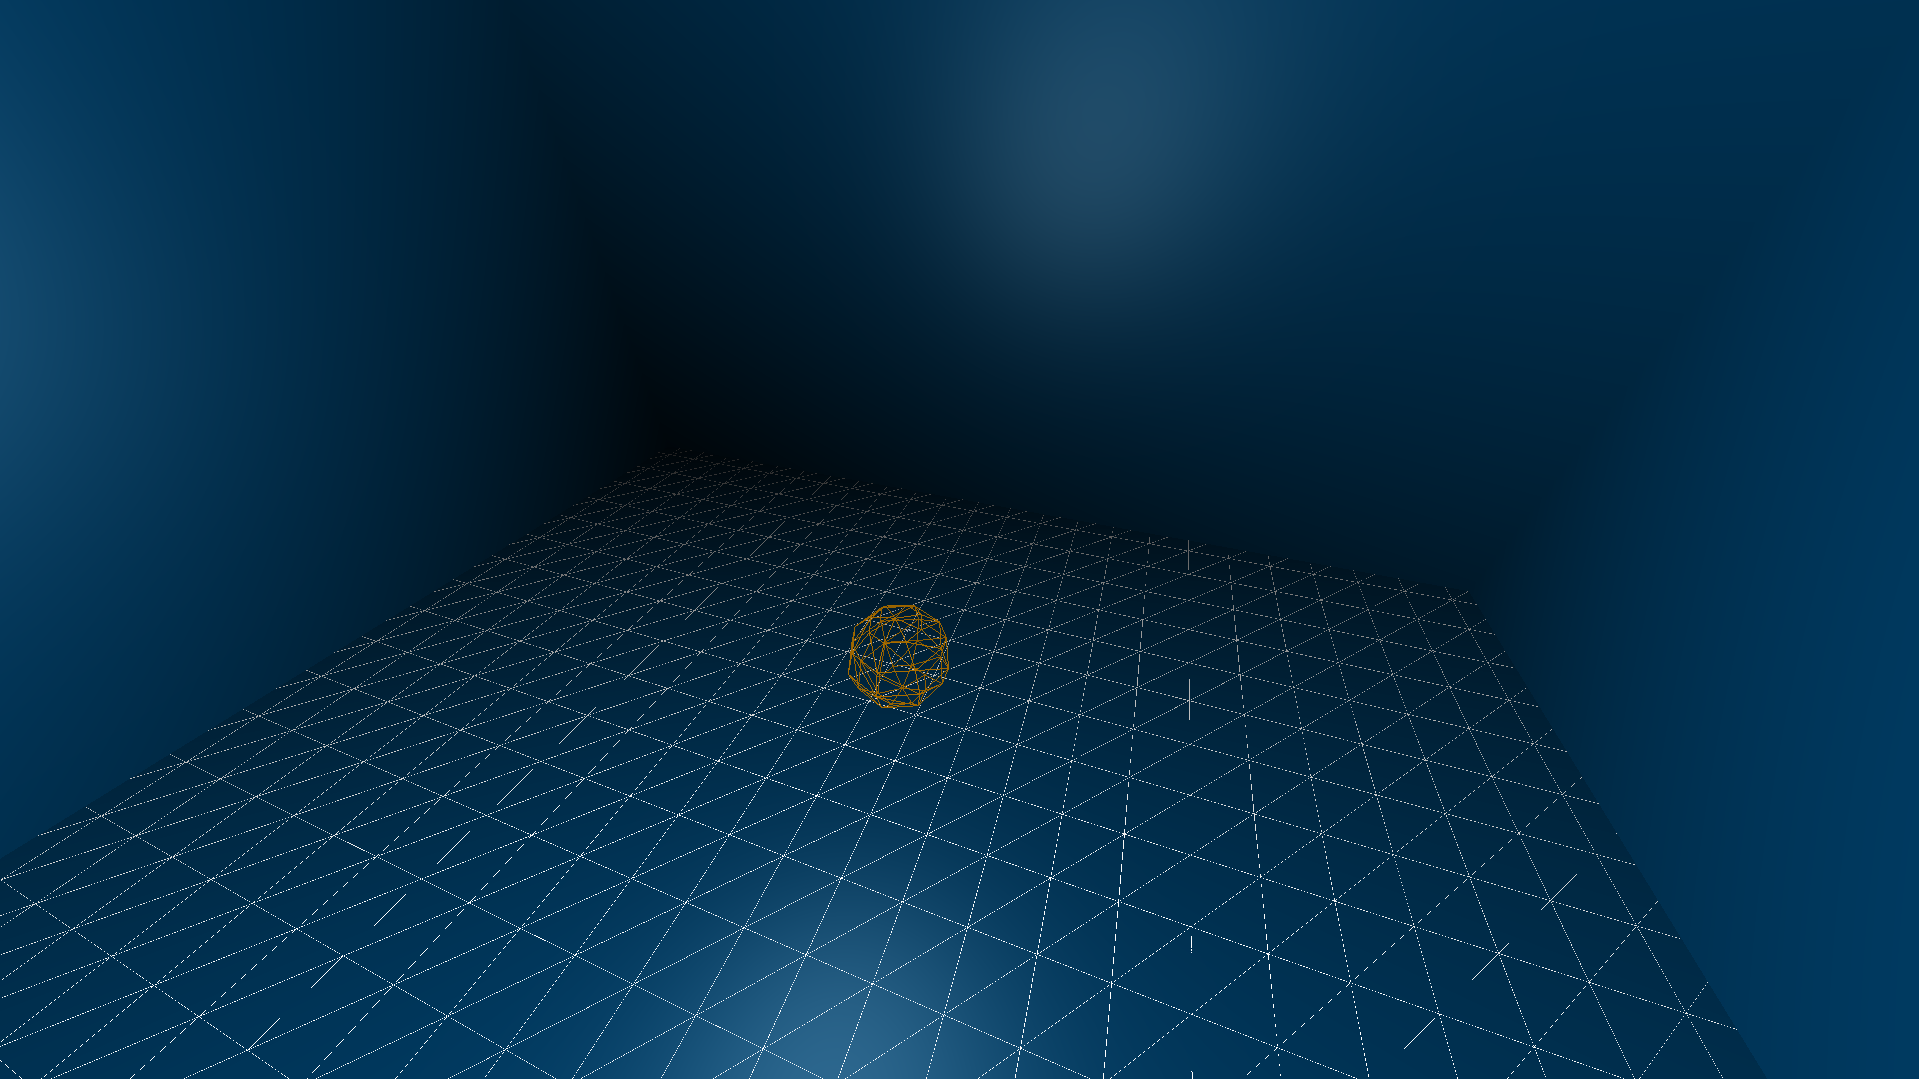
\includegraphics[width=\linewidth]{images/CannonjsDrop.png}
    


\section{What we have left}
\subsection{Scene Environments}
Our current home room has a spinning cube in it from our initial testing.  We want to spiff it up with doors that navigate between each experiment.
\subsubsection{Asset acquisition}
We will be building or buying models to replace the placeholders that we have.
\subsubsection{3D Modeling}
Though some 3D modeling has already been done, more assets are needed for the experiences we plan to create in the coming weeks.
\subsection{Immersive Input}
\subsubsection{Single Controller}
We are currently working on implementing teleportation controls for both single and dual controller movement.
\subsubsection{Dual Controller}
Dual controller controls will use a teleportation control scheme similar to single controller controls.
\subsubsection{Gaze}
We want the app to work with basic "cardboard" virtual reality devices, which don't have a controller. The way we've decided to support these devices is to allow users to select objects by looking at them for an extended period of time. 
\subsection{Object Interaction}
We want a few generic object interactions like teleport and drag and drop, as well as specific interactions for each experiment.
\subsubsection{Raycast Selection}
Once each XR input device has been rendered into the scene, the user needs a way to interact with objects. A raycaster will be used to project a ray out the front of the rendered input device and used to calculate intersections with objects in the scene.
\subsubsection{Drag and Drop}
We need to support picking up objects and placing them down other places, so that users can reposition the objects and observe their interactions. 
\subsection{Physics Simulations}
\subsubsection{Planets Demo}
The planets demo has the core physics complete, but there are still several features we want to add. We want to add user interaction for pausing the simulation and viewing stats of a given planet. We also want to be able to add and remove planets from the system from within the simulation.
\subsubsection{Pendulum Mechanics}
The pendulum has yet to swing in a physically realistic way.  and needs to be able to be carried between tables.
\subsubsection{Core Kinematics}
So far, the experience is just a simple room with the basics of Cannon.js set up to create a ball that just falls to the floor. The goal is to create a sort of playground where the user can spawn in a variety of objects and be able to play around with them in a controllable environment. The user should eventually be able to change the laws of physics by manipulating gravity.
\subsubsection{Laser Refraction}
The refraction of light through certain materials is something we are interested in demonstrating on this site. Specifically, we want to provide an interactive laser refraction chamber to show how light behaves when it penetrates different materials. This experience has not been started yet. and requires assets, raycast input and light refraction equations.x
\subsection{Final Deployment to 01.org}
The last thing we need to do is deploy our site on 01.org, Intel's open source site. 

\section{Problems and Solutions}

% Changing implementation in chrome -> Watching when our devices update + looking at the Chrome change logs
% API changes
\subsection{API instability}
Since we are working with an API that is still in development, changes are to be expected. These changes create an instability in the API which has at times resulted in our code breaking. The only real solution to this is to stay up to date on the changes made to the API and implement any refactoring that needs to be done to our own code in response to these changes. Thankfully, the immersive web group keeps their git repositories and API reference page up to date with all changes. 
% Browser compatibility

% Issues differentiating between scroll to access descriptionary content -> Separate information page
\subsection{Scroll in the same page as VR experience}
One of the repeating problems we have been having is that scroll bars on the VR page cause our canvas to take up slightly more space than the page has, so there is a small amount of awkward scrolling when using the site. After struggling with this for a while, we have decided the best and most logical path forward is to move the content below our canvas, which introduces and links to each of the physics simulations, to a home page. This way, we can have our VR experience take up the entire page and we don't need to worry about scrolling at all. To us, this also seems like a more intuitive user experience.

% Deciding on sprint goals? -> pre-sprint research?

\subsection{Compatibility with other browsers}
Though we initially wrote of our site being compatible with a multitude of browsers, we quickly discovered that due to the nature of the WebXR API, this is simply not possible. Currently, the API is only compatible with the newest versions of Chrome Dev/Canary. Any user visiting the site from browsers other than these will not be able to get the full immersive XR experience. Fortunately, we have been working to add traditional controls to the site in the event that a user is unable to enter the immersive XR modes. For desktop computers without a connected HMD, mouse and keyboard controls have been added. Mobile devices have been given touch controls.

\end{document}